\chapter{Introducción}
\section{Motivación}
En México la comunicación es un derecho fundamental para todas las personas. Sin embargo, las personas de la comunidad sorda enfrentan barreras para poder comunicarse de manera efectiva. Si bien la Lengua de Señas Mexicana (LSM) es el principal medio de comunicación para las personas con discapacidad auditiva en México, en interacciones cotidianas o en situaciones de emergencia, las personas dependen de soluciones tecnológicas para poder comunicarse. Existen pocas herramientas digitales que permiten la traducción de español a LSM, pero en su mayoría no son precisas y muestran animaciones fragmentadas que dificultan la comprensión de los mensajes.\\

La motivación de este Trabajo Terminal es mejorar la accesibilidad de las personas sordas, a la par que se fomenta la inclusión social y tecnológica para esta comunidad, empleando técnicas de Inteligencia Artificial, Procesamiento de Lenguaje Natural y Modelado 3D para obtener una traducción más fluida y natural.

\section{Problemática}
La comunicación es una habilidad esencial que permite a los seres humanos poder interactuar con su entorno y compartir ideas a través de un sistema de símbolos [1]. No obstante, a menudo hay barreras en la comunicación que limitan el acceso a la información y dificultan la capacidad de las personas para expresarse y comunicarse [2]. \\

A pesar de las barreras, las personas sordas han desarrollado su propio medio de comunicación que les permite superar las limitaciones fisiológicas y establecer una conexión efectiva con quienes comparten este lenguaje. En el caso de México, la Lengua de Señas Mexicana (LSM) es el principal medio de comunicación para las personas sordas en el país. \\

Se estima que en el territorio nacional hay un registro de 2.3 millones personas con esta discapacidad [3], lo que evidencia la magnitud de la población que depende de este lenguaje para interactuar en su entorno. Esta lengua posee su propia sintaxis, gramática, léxico y está compuesta por una combinación de señas, expresiones faciales y movimientos corporales que permiten transmitir ideas, mensajes, emociones y sentimientos [4].


\section{Objetivos}
\subsection{Objetivo General}
Desarrollar un prototipo de aplicación móvil en Android que, utilizando técnicas de Procesamiento de Lenguaje Natural y Modelado 3D, traduzca oraciones específicas empleadas en situaciones de emergencia, así como expresiones cotidianas como saludos y agradecimientos, del español a la Lengua de Señas Mexicana (LSM).


\subsection{Objetivo Especifícos}
\begin{itemize}
 \item Desarrollar el módulo de procesamiento de texto mediante técnicas de procesamiento de lenguaje natural, para interpretar oraciones específicas en español y transformarlas en sentencias manipulables para la traducción a la Lengua de Señas Mexicana (LSM).
    \item Construir un módulo de generación de animaciones 3D que represente visualmente las señas en Lengua de Señas Mexicana (LSM), a partir de las oraciones procesadas.
    \item Implementar el módulo de animación y transiciones fluidas utilizando Inteligencia Artificial, con el fin de optimizar significativamente la fluidez entre las señas, buscando una representación natural y continua del lenguaje de señas en los avatares.
    \item Crear una aplicación móvil en Android que integre los módulos de procesamiento de lenguaje natural, generación de avatares y transiciones fluidas entre los componentes del prototipo.
    \item Validar la funcionalidad y usabilidad de la aplicación móvil mediante pruebas con personas con discapacidad auditiva y personas oyentes, en escenarios simulados de emergencia, evaluando la precisión de la traducción y la fluidez de las animaciones.
\end{itemize}

\section{Alcance}
\subsection{Alcance Genral}
El TT consiste en el desarrollo de un prototipo de aplicación móvil que traduzca frases de español a LSM mediante animaciones 3D. La aplicación tendrá un conjunto predefinido de frases comunes para saludos y situaciones de emergencia, y en caso de no contar con una frase específica, se empleará la dactilología (representación de las letras de una palabra empleando las manos) para poder garantizar la comunicación.

\subsection{Alcance Especifíco}
Se hará uso de una interfaz de usuario simple e intuitiva, que sea de utilidad para la población objetivo. Mediante técnicas de Procesamiento Natural. Se pretende hacer un procesamiento del dataset que contiene las frases en español, para posteriormente realizar el modelado de las animaciones 3D empleando Mediapipe; dichas animaciones serán fluidas para mostrar una comunicación natural y fácil de entender.

\subsection{Delimitación}
Es importante aclarar que la traducción será únicamente de un canal de comunicación: de español a LSM. Lo anterior por la razón de que la traducción de LSM a español es más compleja por las diferencias estructurales y gramaticales entre ambos lenguajes.


\section{Justificación}
En México la comunicación inclusiva es un reto para las personas con discapacidad auditiva, debido a que la mayoría de la población no conoce la Lengua de Señas Mexicana (LSM), lo que condiciona a la comunidad sorda para poder expresar sus ideas y pensamientos, acceder a servicios esenciales o recibir apoyo en situaciones de emergencia. Pese a que ha habido avances tecnológicos a lo largo de los últimos años, las herramientas de traducción de español a LSM existentes presentan limitaciones, siendo las más importantes la falta de fluidez en las animaciones y la incompatibilidad entre versiones del sistema operativo de Android.\\

Este Trabajo Terminal busca desarrollar un prototipo de aplicación móvil que traduzca frases en español a LSM con animaciones en 3D fluidas, empleando técnicas de Procesamiento de Lenguaje Natural (PLN) y modelado 3D. Esto tiene el objetivo de contribuir a la accesibilidad, eliminar barreras de comunicación y fomentar la comunicación inclusiva entre personas oyentes y personas con discapacidad auditiva.\\ 

Se espera que este desarrollo sirva de referencia para sentar las bases de futuras investigaciones relacionadas a la traducción e interpretación de lenguas de señas empleando técnicas de Inteligencia Artificial (IA).

\section{Propuesta de solución}
Este proyecto consiste en desarrollar un prototipo que aborde estos problemas, centrándose en la fluidez y precisión de las animaciones de LSM, mediante Inteligencia Artificial, y apoye la interacción entre personas oyentes y personas con discapacidad auditiva mediante Lengua de Señas Mexicanas (LSM), empleando técnicas de procesamiento de lenguaje natural y modelado 3D. El traductor estará enfocado en un conjunto limitado de frases predefinidas, como expresiones de emergencia, saludos y agradecimientos. En caso de no encontrar la frase deseada, el sistema procederá a deletrear la palabra o frase mediante el alfabeto de la Lengua de Señas Mexicanas (LSM), asegurando siempre una respuesta en la comunicación.\\

El prototipo estará diseñado para la última versión de Android, debido a que este es el sistema operativo más utilizado en México [5], por lo que la solución propuesta tendrá un mayor alcance y beneficiará a una mayor cantidad de usuarios. Según diversas estadísticas [5], la penetración de dispositivos Android supera con creces a la de iOS.\\

Para el desarrollo del prototipo se utilizará Media Pipe [6], una biblioteca eficiente para procesamiento de gestos y movimientos corporales, ideal para capturar de manera precisa los gestos de la Lengua de Señas Mexicana. Esto permitirá obtener datos precisos de las señas, garantizando una traducción más confiable y fluida, mientras se mantiene un rendimiento óptimo incluso en dispositivos de gama media.\\

Además, el uso de aplicaciones de Procesamiento de Lenguaje Natural (PLN) es fundamental para el procesamiento del español a LSM, ya que permitirá que el sistema no solo reconozca palabras aisladas, sino también frases y oraciones completas, adaptando la traducción al contexto y mejorando la comunicación en situaciones más complejas.\\

Por otro lado, se busca crear representaciones visuales en 3D para poder facilitar la visualización de señas. Las personas con discapacidad auditiva podrán visualizar una animación asociada a una de las frases que están incluidas dentro del prototipo.
\newline

\textbf{Productos Esperados}
\begin{itemize}
    \item Dataset normalizado de LSM.
    \item Set de animaciones con avatares 3D fluidos e interactivos.
    \item Aplicación móvil en Android.
    \item Documentación del sistema.
\end{itemize}
\begin{center}
    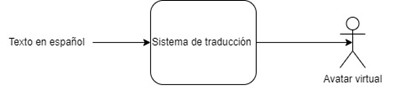
\includegraphics[width=0.8\textwidth]{TT1/Images/diacajanegra.jpg}
    \captionof{figure}{Diagrama del funcionamiento de la App, elaboraci´on propia.}  % Pie de foto manual
\end{center}


\section{Estado del arte}
Se han desarrollado diversas investigaciones y desarrollos de sistemas de software que abordan la problemática de la comunicación entre personas oyentes y no oyentes. A continuación se describen los trabajos relacionados: 
\begin{itemize}
    \item Translation of Spanish Text to Mexican Sign Language Glossed Text Using Rules and Deep Learning. En este trabajo se presenta una arquitectura para traducir de español a Lengua de Señas Mexicana (LSM), cuyos resultados fueron evaluados con las métricas BLEU y WER. En este artículo se encontró que la traducción con técnicas tradicionales tiene un mejor desempeño que el aprendizaje profundo [7].
\item Resource Creation for Automatic Translation System from Texts in Spanish into Mexican Sign Language. Este artículo presenta la creación de recursos lingüísticos para la traducción automática del español escrito a LSM, así como el sistema que la implementa. En colaboración con la Casa de la Cultura de los Sordos (CDMX), se tradujeron 150 oraciones pertenecientes a 13 estructuras gramaticales reconocidas por el sistema, identificando 100 signos que pueden representar una oración completa. Se observó que, ante la falta de un signo específico, las personas sordas tienden a deletrear la palabra. El sistema traduce de forma literal al buscar y reproducir palabras en su base de datos, además de contar con signos que representan expresiones completas [8].
\item Aplicación “Voz y Señas”. Esta aplicación, desarrollada por el Instituto de Pedagogia en conjunto con TecnoPrótesis y Bienestar Incluyente A.C.,  permite traducir la LSM por medio del habla o escribiendo texto. Sus objetivos son favorecer la comunicación entre una persona sorda y una persona oyente, y ser una herramienta auxiliar en los procesos de alfabetización, redacción de textos y comprensión lectora [9]. 
\item Hetah. Servicio en línea que funciona como traductor de Lengua de Señas Colombiana (LSC), que permite la comunicación entre personas oyentes y no oyentes mediante un Avatar 3D. Se debe ingresar la frase que se desea traducir y posteriormente, el avatar realizará la traducción mediante gestos [10]. 
\item SignAloud. Sistema de Inteligencia Artificial que emplea guantes capaces de reconocer gestos de las manos correspondientes a palabras y frases en Lenguaje de Señas Americana. Dichos guantes contienen sensores que registran la posición y el movimiento de las manos, para generar datos que son enviados de forma inalámbrica a una computadora central. La computadora analiza los datos de los gestos empleando redes neuronales, y si los datos coinciden con un gesto, la palabra o frase asociada se pronuncia en un altavoz [11].
\item Sistema traductor de la Lengua de Señas Mexicana mediante dactilología y de español a español signado. Sistema de Inteligencia Artificial capaz de ayudar a entablar un diálogo entre una persona sorda y otra oyente, mediante la traducción de las señas de dactilología a  texto plano en español y de forma análoga, la traducción del texto plano a español a español signado [12].

	

\end{itemize}

\section{Metodología}
El proyecto se desarrollará bajo la metodología Scrum, un marco de trabajo ágil que organiza la colaboración del equipo a través de roles, artefactos y reglas que garantizan su correcta implementación [13][14]. Uno de sus principios clave es la configuración de equipos autogestionados y multifuncionales, lo que permite tomar decisiones autónomas sin depender de directrices externas [14].\\

La estructura de Scrum se basa en ciclos iterativos llamados Sprints, en los cuales se genera un incremento funcional del producto. Cada Sprint se gestiona como un proyecto independiente con objetivos específicos [14]. Además, estos ciclos incluyen cinco elementos clave: reunión de planeación, Daily Scrum, trabajo de desarrollo, revisión del Sprint y retrospectiva del Sprint, asegurando así una mejora continua en cada iteración. Para este desarrollo, los Sprints tendrán una duración de entre dos y cuatro semanas, lo que facilitará una transición progresiva hacia esta metodología y garantizará un avance constante.\\

Otro punto a destacar es que Scrum define tres roles esenciales. En primer lugar, el Scrum Master guía la implementación de la metodología y facilita la resolución de impedimentos sin gestionar directamente el desarrollo [15]. En segundo lugar, el Product Owner representa a los interesados y gestiona el Product Backlog, priorizando las funcionalidades para maximizar el valor del producto [15]. Por último, el equipo de desarrollo transforma estos requerimientos en incrementos funcionales, operando sin jerarquías y con un tamaño ideal de tres a nueve integrantes [15].\\

En este proyecto, el equipo asumirá exclusivamente el rol de desarrolladores, encargándose de transformar los requerimientos en incrementos funcionales del producto. La estructura del equipo se distribuirá en tres áreas especializadas. El desarrollador de animaciones 3D y MediaPipe diseñará avatares, implementará gestos y optimizará las transiciones. El desarrollador de Android estructurará la aplicación, desarrollará interfaces y conectará los módulos. Por su parte, el desarrollador de PLN implementará el procesamiento de lenguaje natural, adaptará las frases al contexto de LSM y optimizará la comunicación con los módulos de animación.\\

Esta distribución permitirá aplicar Scrum de manera eficiente, asegurando un desarrollo iterativo y coordinado, en el que cada integrante contribuirá activamente al avance del proyecto mediante la integración de sus respectivas áreas.


\begin{center}
    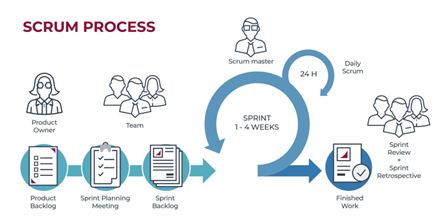
\includegraphics[width=0.8\textwidth]{TT1/Images/metoscrum.png}
    \captionof{figure}{Metodología Scrum, obtenido de [].}  % Pie de foto manual
\end{center}
